\chapter{面向应急车辆的“绿波带”模型}
\label{ch3}

本章将要介绍面向应急车辆优先通行的“绿波带”模型、本文信号控制方法的系统架构、系统各部分工作流程图以及整体思路算法。

\section{“绿波带”模型}
本文将整个路网建模为由交叉口和路段所构成的有向图${G(I, E)}$,路口抽象为图的顶点,路段抽象为图的边,其中${I}$表示顶点集和,即交叉口以及起点和终点的集和。${E}$表示边集和,即路段集和,边由相邻顶点构成,如${e_1=(I_1, I_2)}$,代表${e_1}$的起点为${I_1}$终点为${I_2}$。应急车辆接收到任务后获取到最快路径,本文将最快路径构建为“绿波带”模型,“绿波带”模型表示为${p=I_0\rightarrow I_1\rightarrow\ldots\rightarrow I_n}$,其中${(I_i, I_i+1) \in E, \forall i \in 1, 2, \ldots, n-1}$,如图\ref{fig:path}所示,应急车辆预计到达路口${I_i}$的时间记为${t_i}$,其中${I_0}$和${I_n}$分别代表起点和终点,因此${t_0=0}$,为应急车辆出发的时刻。${t_n}$为应急车辆到达目的地的时刻,即旅行时间。


\begin{figure}[H]
	\centering
	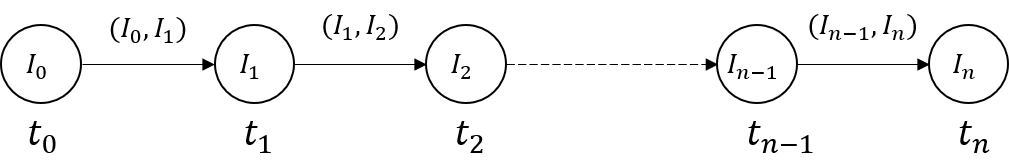
\includegraphics[width=\textwidth]{figures/path.png}
	\caption{由连续节点表示的“绿波带”模型}
	\label{fig:path}
\end{figure}

本文中交通路口${I_i}$的智能交通灯由一个非集中式的智能体${AGT_i}$控制,定义${AGT=\left\{ {AGT_1, AGT_2, \ldots , AGT_i, \ldots, AGT_{n-1}} \right\}}$,每个智能体${AGT_i}$控制着交通路口${I_i}$的所有交通灯,因此智能体${AGT_i}$与交通路口${I_i}$一一对应,应急车辆最快路径上的智能体模型如图\ref{fig:agent}所示。

\begin{figure}[H]
	\centering
	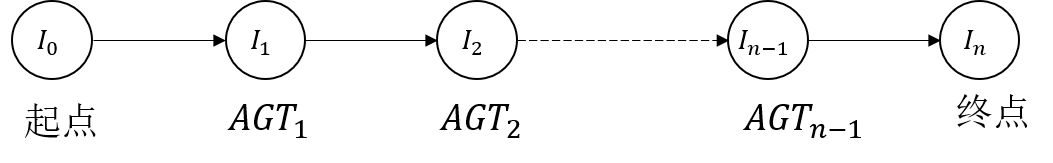
\includegraphics[width=\textwidth]{figures/agent.png}
	\caption{路口与智能体对应关系}
	\label{fig:agent}
\end{figure}

应急车辆预计到达交通灯路口${I_i}$的时间${t_i}$至关重要,它在第\ref{ch4}章起着关键性的作用。本文中,应急车辆在行使的过程中,由于道路饱和度的降低以及信号抢占策略,应急车辆能够快速且平稳地行驶,且不会在交通灯路口停止,因此预计到达时间${t_i}$不考虑在路口停留时间,只跟应急车辆的速度和应急车辆与路口${I_i}$的距离有关。为了贴近实际物理场景,本文中应急车辆的速度在${[v-\delta_{spd}, v+\delta_{spd}]}$范围内变化,其中${v}$为应急车辆在一段行驶时间内的平均速度,由于应急车辆不受道路限速的影响,且应急车辆应以尽可能快的速度行驶,本文设置${v}$的最大值为道路限速的1.5倍,${\delta_{spd}}$表示应急车辆在行驶过程中速度的偏差,取值为${v}$的0.2倍。我们用${s_i^t}$表示当前时刻${t}$应急车辆到达前方交通灯路口${I_i}$的距离,应急车辆到达交通灯路口${I_i}$的预计到达时间为

\begin{equation}
	t_i= t + \frac{s_i^t}{v} 
	\label{equation:t_i}
\end{equation}

由于应急车辆受到周围环境的影响,其速度不是固定值,因此预计到达时间不应该为固定值,本文根据\cite{min}中的方法,采用预计到达时间范围来表示应急车辆到达的时间范围,使预计到达时间在${[t_i-\delta_i, t_i+\delta_i]}$之间,其中${\delta_i}$为应急车辆预计到达路口${I_i}$的时间偏差,${\delta_i}$的值与应急车辆速度变化范围以及时刻${t}$应急车辆与交通灯路口${I_i}$的距离${s_i^t}$有关,${t_i-\delta_i}$为最快到达时刻,${t_i+\delta_i}$为最慢到达时刻。${\delta_i}$表示为

\begin{equation}
	\delta_i=\frac{\frac{s_i^t}{v-\delta_{spd}}-\frac{s_i^t}{v+\delta_{spd}}}{2}=\frac{s_i^t\times\delta_{spd}}{v^2-\delta_{spd}^2}
	\label{equation:delta_i}
\end{equation}

式中${\delta_{spd}}$表示应急车辆在行驶过程中速度的偏差,${\mu_t-\delta_{spd}}$为应急车辆在行驶过程中的最小速度,${v+\delta_{spd}}$为应急车辆在行驶过程中的最大速度。当预计到达时间确定之后,就不需要重复计算,因为预计到达时间一定在${[t_i-\delta_i, t_i+\delta_i]}$范围内。

\section{系统架构}
面向应急车辆优先通行的交通信号灯智能控制方法的系统架构如图\ref{fig:architecture}所示,当应急车辆接收到紧急任务后,首先获取最快路径,然后获取最快路径上的交叉口,并与所有的交叉口智能体进行通信。途径的交叉口${I_1 \to I_2 \to \ldots \to I_n}$构成了最快路径,每一个交叉口${I_i}$有与之对应的智能体${AGT_i}$。应急车辆实时地与最快路径上的所有交叉口智能体通信。智能体控制该交叉口的所有交通信号灯,交通信号灯在智能体的控制下进入降低道路饱和度、信号抢占以及恢复交通流阶段。应急车辆与最快路径上的所有智能体并行通信,直到应急车辆通过该智能体对应的交叉口之后才终止通信。

\begin{figure}[ht]
	\centering
	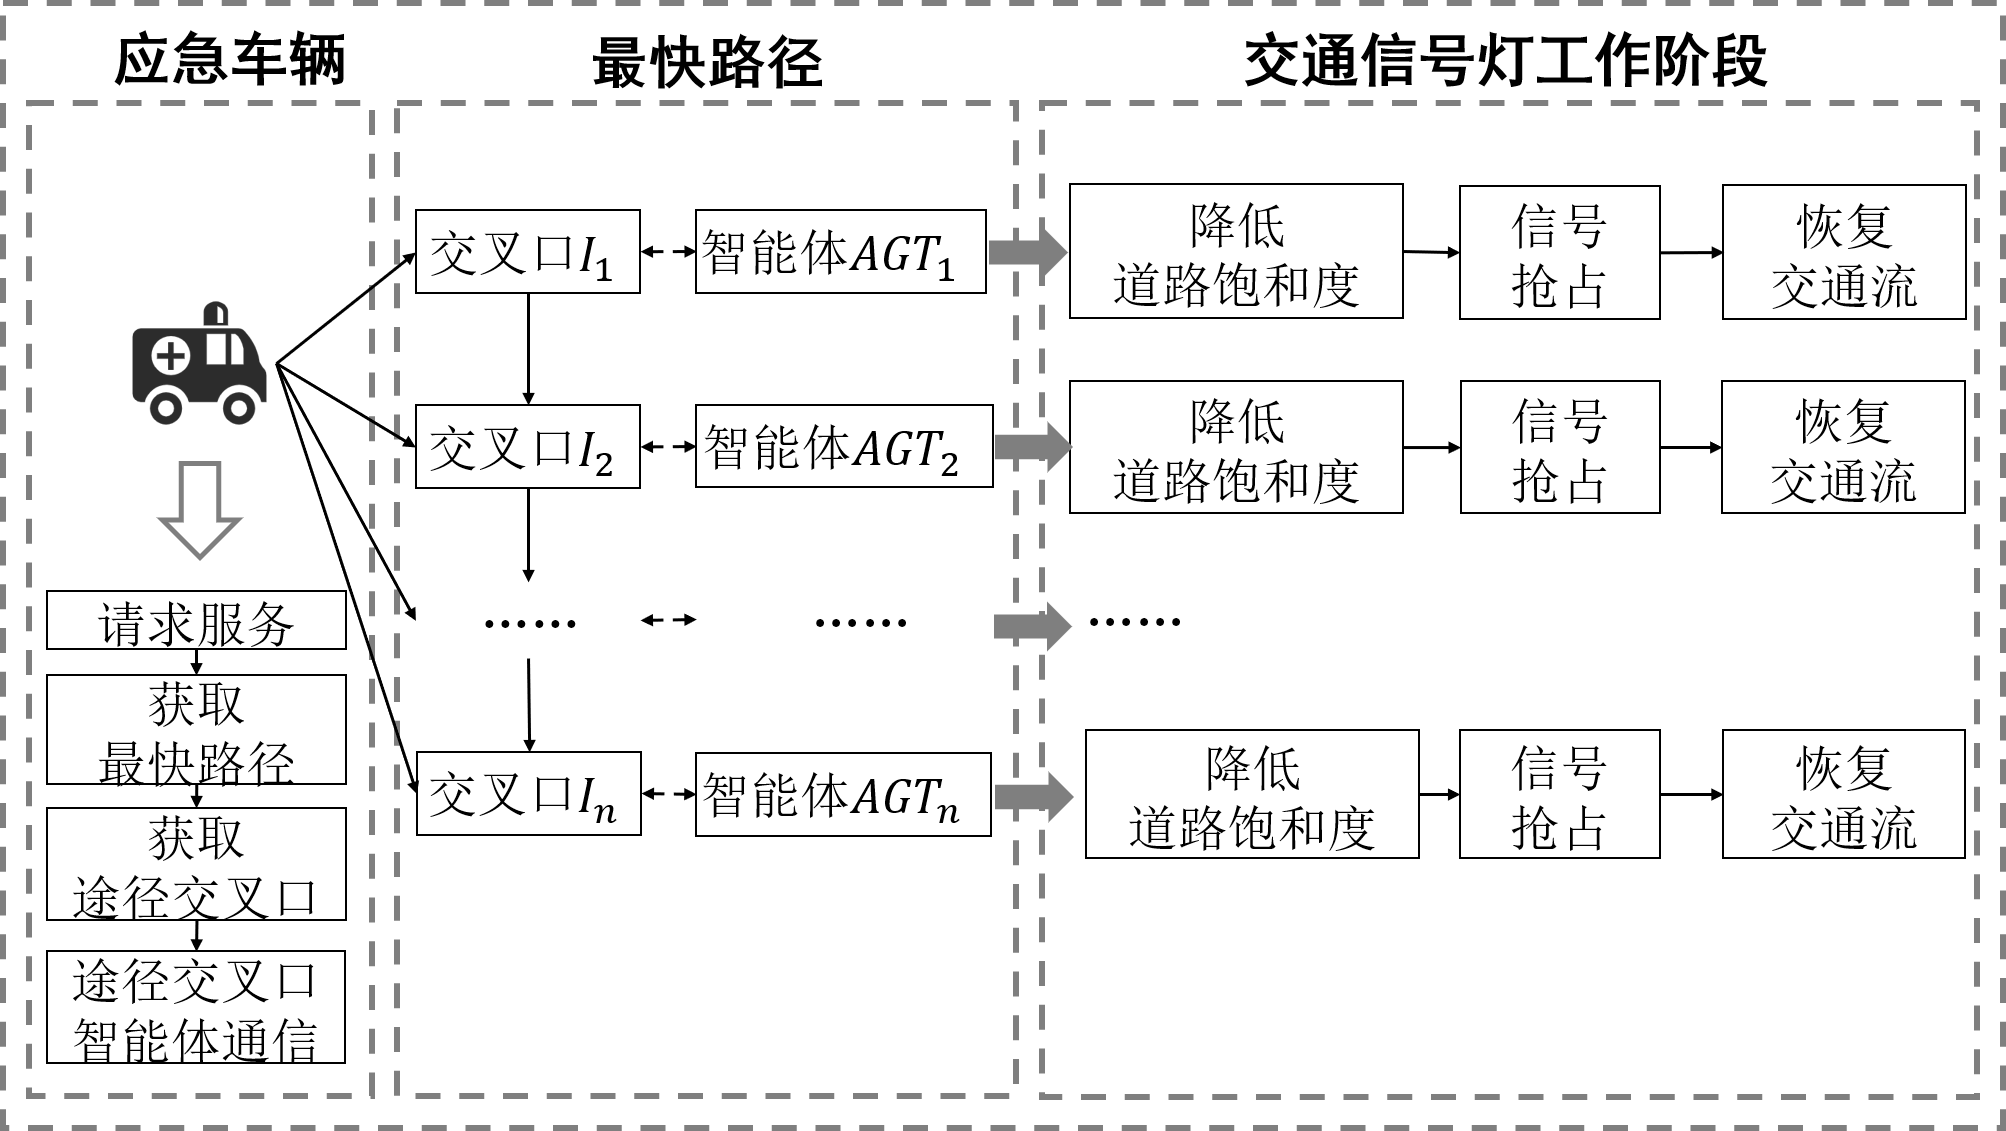
\includegraphics[width=\textwidth]{figures/architecture.png}
	\caption{系统架构}
	\label{fig:architecture}
\end{figure}

应急车辆、交叉口智能体以及交通信号灯的工作流程如图\ref{fig:kuangjia}所示。应急车辆接受到紧急任务后,获取最快路径,并向最快路径上所有交通路口智能体发送应急车辆的速度${v}$、速度偏差${\delta_{spd}}$、应急响应等级(Emergency Response Level,简称ERL)以及GPS,并在接下来的行程中,保持与智能体的联系,直至通过智能体所在交叉口。交叉口智能体通过降低道路饱和度算法、非侵入式信号抢占算法、侵入式信号抢占算法,使得交通信号灯在未请求阶段、降低道路饱和度阶段、信号抢占阶段以及恢复交通流阶段之间过渡。交通信号灯在智能体的控制在以下四个阶段之间过渡:

\begin{enumerate}
	\item 未请求阶段:没有应急车辆请求条件下的阶段;
	\item 降低道路饱和度阶段:在应急车辆请求条件下,为应急车辆的到来降低目标相位对应车道饱和度的阶段;
	\item 信号抢占阶段:为应急车辆提供绿灯指引的阶段;
	\item 恢复交通流阶段:为降低应急车辆优先对整个交通流造成的负面影响以及过渡到未请求阶段。
\end{enumerate}

\begin{figure}[ht]
	\centering
	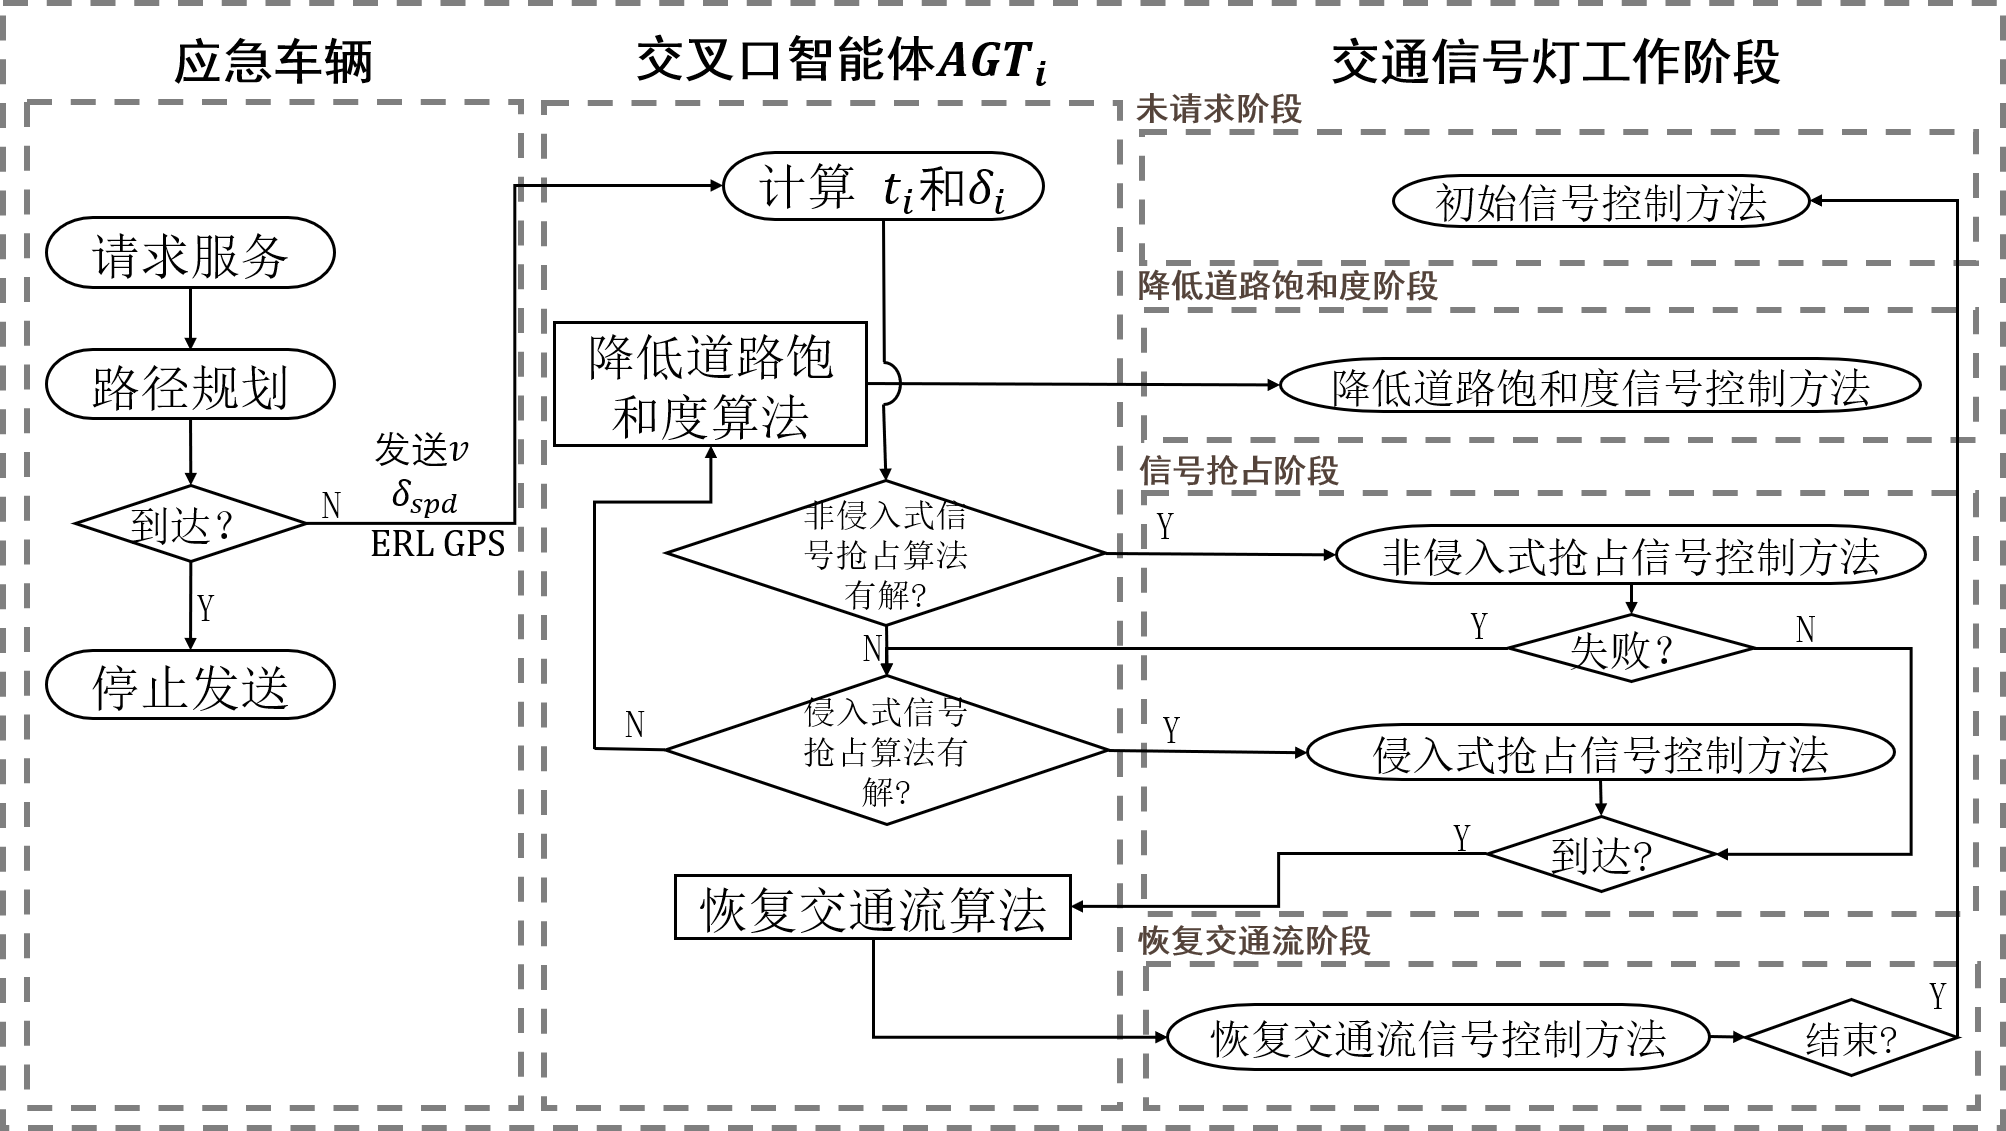
\includegraphics[width=\textwidth]{figures/kuangjia.png}
	\caption{系统各部分工作流程图}
	\label{fig:kuangjia}
\end{figure}



%\begin{figure}[ht]
%	\centering
%	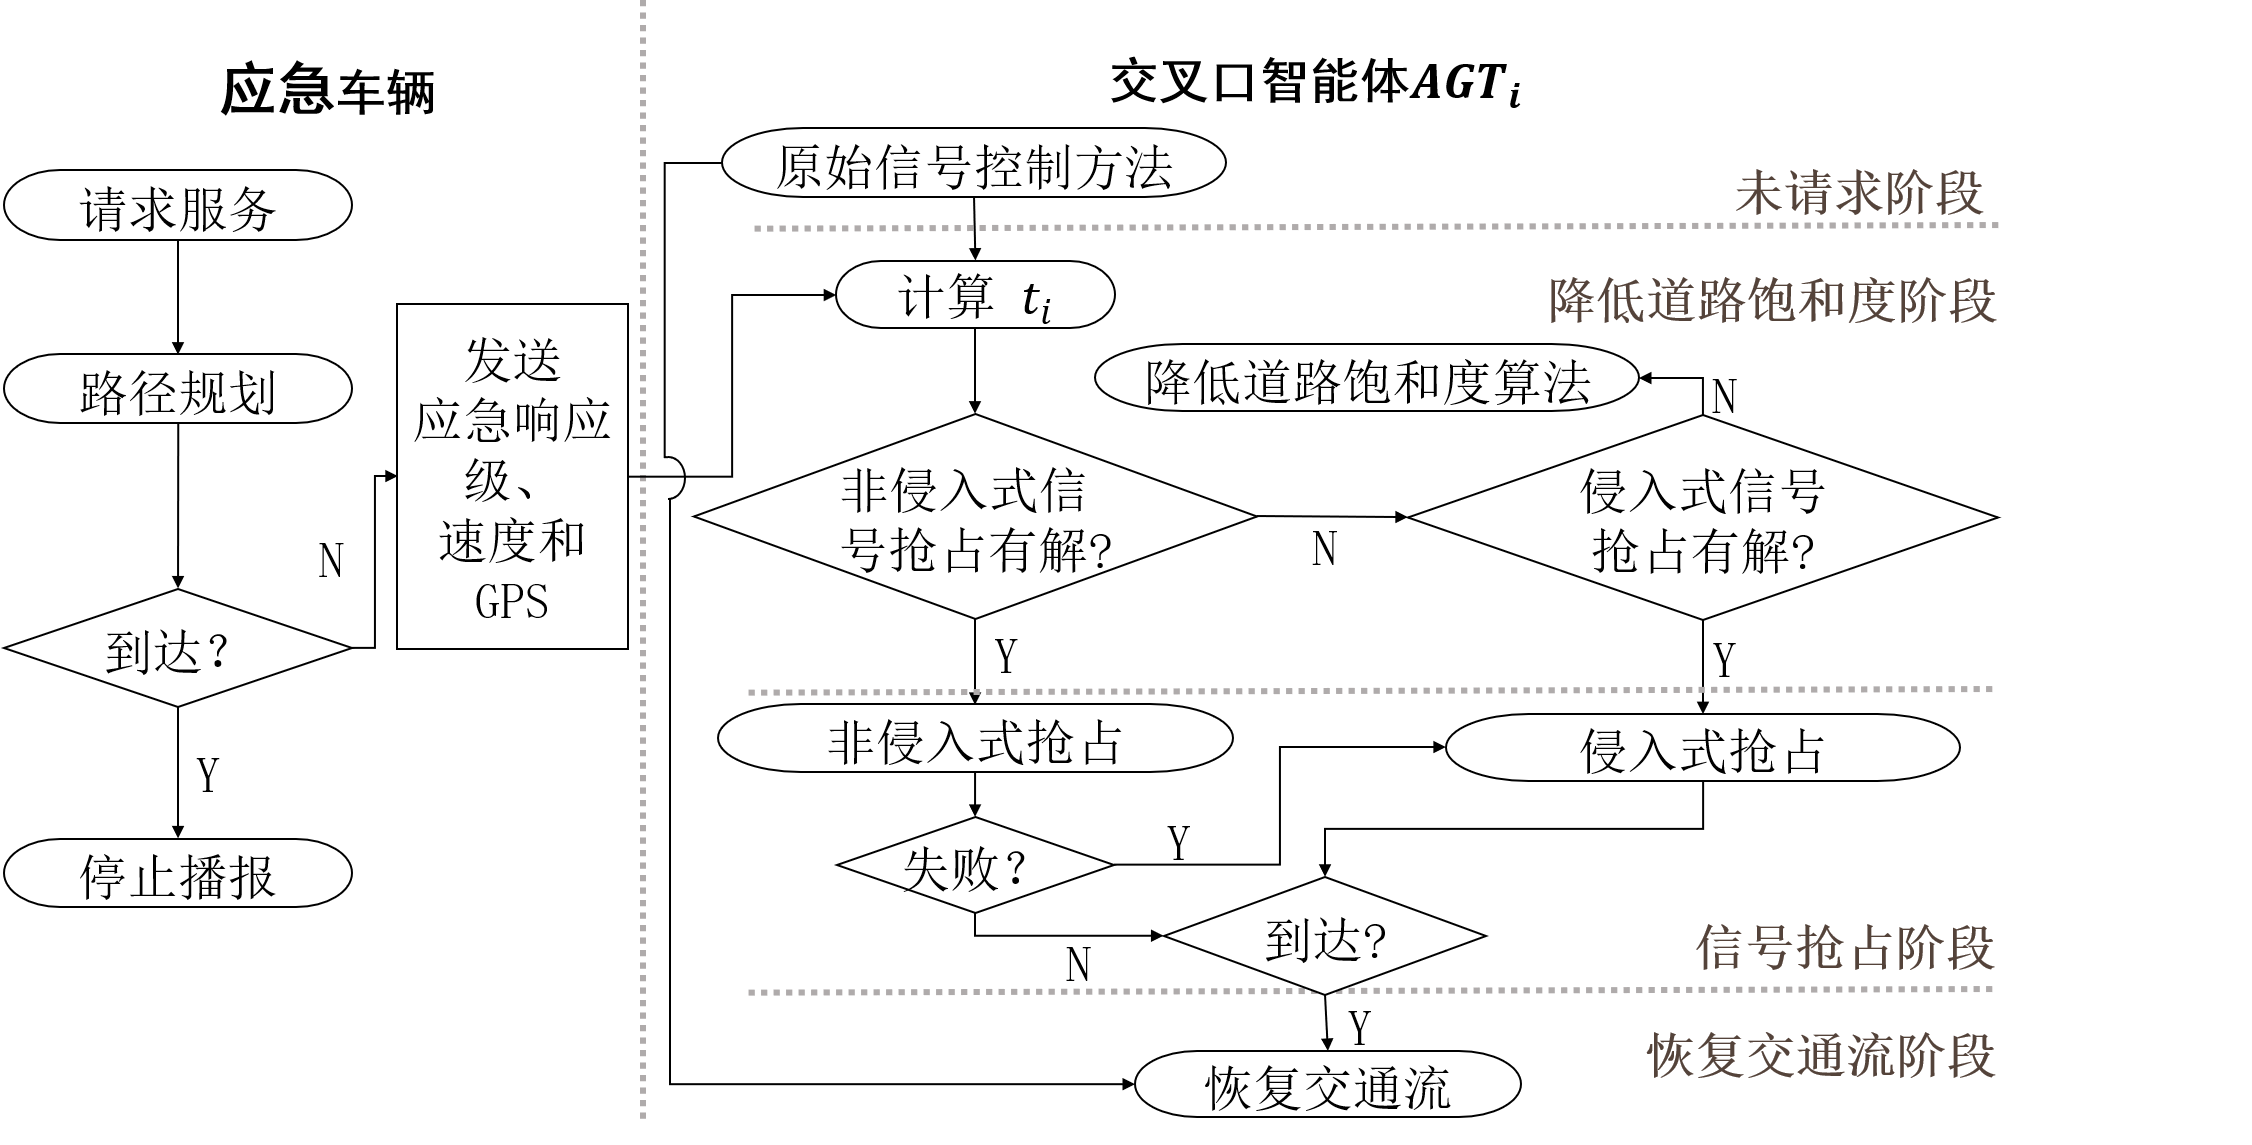
\includegraphics[width=\textwidth]{figures/workflow.png}
%	\caption{智能体控制交通灯流程图}
%	\label{fig:workflow}
%\end{figure}

交叉口智能体${AGT_i}$的工作流程如图\ref{fig:kuangjia}所示。交叉路口智能体${AGT_i}$接收到应急车辆的请求后,根据接收到的${v}$、速度偏差${\delta_{spd}}$以及GPS信息计算出应急车辆到达交叉口${I_i}$的预计到达时间${t_i}$以及时间偏差${\delta_{i}}$。智能体${AGT_i}$通过非侵入式信号抢占算法计算出非侵入式信号抢占算法是否有可行解,若不存在可行解,智能体${AGT_i}$通过侵入式信号抢占算法计算出侵入式信号抢占算法是否有可行解,若依然不存在可行解,则智能体${AGT_i}$通过降低道路饱和度算法计算出降低道路饱和度的信号控制方案,使得该路口交通信号灯从使用初始信号控制方法的未请求阶段过渡到降低道路饱和度阶段,采用降低道路饱和度的信号控制方法。当非侵入式信号抢占算法或者侵入式信号抢占算法有可行解时,则使得交通信号灯从原来的阶段过渡到信号抢占阶段,若非侵入式信号抢占算法有可行解,则优先采用非侵入式信号抢占方法,侵入式信号抢占方法作为兜底措施,保证应急车辆快速通过交叉路口而无需停车和降速。当应急车辆通过交叉路口后,智能体通过恢复交通流算法,计算出恢复交通流阶段的各信号相位时长,恢复交通流阶段的信号控制方案能够使得交通流在最快的时间内恢复。交通灯从信号抢占阶段过渡到恢复交通流阶段。当恢复交通流阶段的信号周期执行结束,交通信号灯回到未请求阶段,采用初始的信号控制方法。


%确保应急车辆到达交叉口时,前方无排队车辆,且应急车辆前方为绿灯。当应急车辆通过交叉口后,智能体通过恢复交通流算法,计算出恢复交通流阶段的各信号相位时长,恢复交通流阶段的信号控制方案能够使得交通流在最快的时间内恢复。交通灯从信号抢占阶段过渡到恢复交通流阶段。当恢复交通流阶段的信号周期执行结束,交通信号灯回到未请求阶段,采用初始的信号控制方法。

\section{算法描述}
伪代码如算法如\ref{alg}所示,算法的输入为${v}$, ${\delta_{spd}}$, ERL, GPS。输出为交通信号灯采取的信号控制方法,包含了初始信号控制方法、降低道路饱和度信号控制方法、非侵入式抢占信号控制方法、侵入式抢占信号控制方法以及恢复交通信号控制方法。当交叉口智能体${AGT_i}$接收到应急车辆的请求后,根据交通信号灯所在的阶段执行不同的算法。

\begin{enumerate}
	\item 当交通信号灯处于未请求阶段或者降低道路饱和度阶段,计算非侵入式抢占算法是否能够得到可行解以及侵入式抢占算法的最迟抢占时间,若非侵入式抢占算法有可行解,则交通信号灯过渡到信号抢占阶段,并采用非侵入式抢占信号控制方法;若非侵入式抢占算法没有可行解,而侵入式抢占算法有可行解,则交通信号灯过渡到信号抢占阶段,并采用侵入式抢占信号控制方法;若非侵入式抢占算法和侵入式抢占算法都没有可行解,则交通信号灯采取降低道路饱和度信号控制方法;
	\item 当交通信号灯处于信号抢占阶段,若交通信号灯正在采用非侵入式抢占信号控制方法,但是非侵入式抢占失败,则需要重新规划非侵入式信号抢占方案,若非侵入式抢占算法有可行解,则更新非侵入式抢占信号控制方法的信号配时,否则,交通信号灯采用侵入式抢占信号控制方法;若应急车辆通过了交叉口,则交通信号灯采取恢复交通信号控制方法;
	\item 当交通信号灯处于恢复交通流阶段,当前恢复周期执行结束后,过渡到未请求阶段,交通信号灯采用初始信号控制方法。
\end{enumerate}

 %控制交通灯降低道路饱和度进入降低道路饱和阶段,在该阶段中, 首先智能体判断非侵入式信号抢占策略是否能够得出最优解,若能够得出最优解,智能体控制信号灯进入信号抢占阶段,若不能得出最优解,智能体判断是否需要进行侵入式信号抢占,若需要则进入到信号抢占阶段,否则交通灯依然保持在降低道路饱和度阶段;在信号抢占阶段,智能体控制路口交通灯为应急车辆提供绿灯指引,当应急车辆通过交通路口后,进入恢复交通流阶段;在恢复交通流阶段,智能体通过计算得出恢复方案,在最快的时间内恢复交通流,交通灯回到原本的信号控制方案。

\begin{breakablealgorithm}
	\caption{信号控制算法} 
	\label{alg}
	\begin{algorithmic}[1]
		\REQUIRE ${v}$, ${\delta_{spd}}$, ERL, GPS
		\ENSURE 交通信号灯采取的信号控制方法
		\WHILE {接受到应急车辆的请求}
			\STATE 计算${t_i}$和${\delta_i}$,根据式\ref{equation:t_i}和\ref{equation:delta_i}
		
			\IF {交通信号灯处于未请求阶段 或者 降低道路饱和度阶段}
				\STATE 计算非侵入式抢占算法是否能够得到可行解
				\STATE 计算侵入式抢占算法是否能够得到可行解
				\IF {非侵入式抢占算法有可行解}
					\STATE 交通信号灯进入信号抢占阶段
					\STATE \textbf{return}非侵入式抢占信号控制方法
				\ELSIF{侵入式抢占算法有可行解}
					\STATE 交通信号灯进入信号抢占阶段
					\STATE \textbf{return}侵入式抢占信号控制方法
				\ELSE 
					\IF{交通信号灯处于未请求阶段}
						\STATE 交通信号灯进入道路饱和度阶段
					\ENDIF
					\STATE \textbf{return}降低道路饱和度信号控制方法
				\ENDIF
			\ELSIF {交通信号灯处于信号抢占阶段}
				\IF{交通信号灯正在采用非侵入式抢占信号控制方法}
					\IF{非侵入式抢占信号控制方法失败}
						\STATE 计算非侵入式抢占算法是否能够得到可行解
						\IF {非侵入式抢占算法有可行解}
							\STATE \textbf{return}更新非侵入式抢占信号控制方法
						\ELSE 
							\STATE \textbf{return}侵入式抢占信号控制方法
						\ENDIF
					\ENDIF
					\IF{应急车辆通过交叉口}
						\STATE 交通信号灯进入恢复交通流阶段
						\STATE \textbf{return}恢复交通流信号控制方法
					\ENDIF
				\ENDIF
			\ELSE
				\IF{恢复周期执行结束}
					\STATE 交通信号灯进入未请求阶段
					\STATE \textbf{return}初始信号控制方法
				\ENDIF
			\ENDIF
		\ENDWHILE
	\end{algorithmic}
\end{breakablealgorithm}

\section{本章小结}
本章构建了面向应急车辆优先通行的“绿波带”模型,将交叉口视为结点,路段视为边,每个交叉口都有与之对应的智能体。路网建模完成之后,本文设计了计算到达交叉口预计到达时间的算法,并根据应急车辆速度的动态性将预计到达时间的时间偏差考虑在内。本章还构建了包含应急车辆模块、最快路径模块以及交通信号灯模块的系统架构,并设计了应急车辆、交叉口智能体以及交通信号灯的工作流程。最后本章设计了面向应急车辆优先通信的交通信号灯智能控制方法整体思路算法。
